\documentclass[a4paper,12pt,twoside]{memoir}

% Castellano
\usepackage[spanish,es-tabla]{babel}
\selectlanguage{spanish}
\usepackage[utf8]{inputenc}
\usepackage[T1]{fontenc}
\usepackage{lmodern} % Scalable font
\usepackage{microtype}
\usepackage{placeins}

\RequirePackage{booktabs}
\RequirePackage[table]{xcolor}
\RequirePackage{xtab}
\RequirePackage{multirow}

% Links
\PassOptionsToPackage{hyphens}{url}\usepackage[colorlinks]{hyperref}
\hypersetup{
	allcolors = {red}
}

% Ecuaciones
\usepackage{amsmath}

% Rutas de fichero / paquete
\newcommand{\ruta}[1]{{\sffamily #1}}

% Párrafos
\nonzeroparskip

% Huérfanas y viudas
\widowpenalty100000
\clubpenalty100000

\let\tmp\oddsidemargin
\let\oddsidemargin\evensidemargin
\let\evensidemargin\tmp
\reversemarginpar

% Imágenes

% Comando para insertar una imagen en un lugar concreto.
% Los parámetros son:
% 1 --> Ruta absoluta/relativa de la figura
% 2 --> Texto a pie de figura
% 3 --> Tamaño en tanto por uno relativo al ancho de página
\usepackage{graphicx}

\newcommand{\imagen}[3]{
	\begin{figure}[!h]
		\centering
		\includegraphics[width=#3\textwidth]{#1}
		\caption{#2}\label{fig:#1}
	\end{figure}
	\FloatBarrier
}







\graphicspath{ {./img/} }

% Capítulos
\chapterstyle{bianchi}
\setlength{\headheight}{32pt}
\newcommand{\capitulo}[2]{
	\setcounter{chapter}{#1}
	\setcounter{section}{0}
	\setcounter{figure}{0}
	\setcounter{table}{0}
	\chapter*{#2}
	\addcontentsline{toc}{chapter}{#2}
	\markboth{#2}{#2}
}

% Apéndices
\renewcommand{\appendixname}{Apéndice}
\renewcommand*\cftappendixname{\appendixname}

\newcommand{\apendice}[1]{
	%\renewcommand{\thechapter}{A}
	\chapter{#1}
}

\renewcommand*\cftappendixname{\appendixname\ }

% Formato de portada

\makeatletter
\usepackage{xcolor}
\newcommand{\tutor}[1]{\def\@tutor{#1}}
\newcommand{\tutorb}[1]{\def\@tutorb{#1}}

\newcommand{\course}[1]{\def\@course{#1}}
\definecolor{newBox}{HTML}{D8AD6E}
\def\maketitle{
  \null
  \thispagestyle{empty}
  % Cabecera ----------------
\begin{center}
  \noindent
\includegraphics[width=\textwidth]{CabeceraEPS.png}\vspace{1.5cm}%
\end{center}
  
  % Título proyecto y escudo salud ----------------
  \begin{center}
    \begin{minipage}[c][1.5cm][c]{.20\textwidth}
        \includegraphics[width=\textwidth]{logo_GIS.png}
    \end{minipage}
  \end{center}
  
  \begin{center}
    \colorbox{newBox}{%
        \begin{minipage}{.8\textwidth}
          \vspace{.5cm}\Large
          \begin{center}
          \textbf{TFG del Grado en Ingeniería de la Salud}\vspace{.6cm}\\
          \textbf{\LARGE\@title{}}
          \end{center}
          \vspace{.2cm}
        \end{minipage}
    }%
  \end{center}
  
    % Datos de alumno, curso y tutores ------------------
  \begin{center}%
  {%
    \noindent\LARGE
    Presentado por \@author{}\\ 
    en Universidad de Burgos\\
    \vspace{0.5cm}
    \noindent\Large
    \@date{}\\
    \vspace{0.5cm}
    %Tutor: \@tutor{}\\ % comenta el que no corresponda
    Tutores: \@tutor{} -- \@tutorb{}\\
  }%
  \end{center}%
  \null
  \cleardoublepage
  }
\makeatother

\newcommand{\nombre}{Carmen Ruiz Alonso}
\newcommand{\nombreTutor}{Miriam Saiz Rodríguez} 
\newcommand{\nombreTutorb}{Alicia Olivares Gil} 
\newcommand{\dni}{71188814L} 

% Datos de portada
\title{InteraDD: Herramienta web para la detección e interpretación de interacciones farmacológicas basadas en el sistema CYP450}
\author{\nombre}
\tutor{\nombreTutor}
\tutorb{\nombreTutorb} 
\date{\today}


\begin{document}

\maketitle


\newpage\null\thispagestyle{empty}\newpage

%%%%%%%%%%%%%%%%%%%%%%%%%%%%%%%%%%%%%%%%%%%%%%%%%%%%%%%%%%%%%%%%%%%%%%%%%%%%%%%%%%%%%%%%
\thispagestyle{empty}

\noindent
\includegraphics[width=\textwidth]{CabeceraEPS.png}\vspace{1cm}

\noindent D. \nombreTutor, profesora del departamento de Ciencias de la Salud, área de Fisiología.
\noindent D. \nombreTutorb, profesora del departamento de Ingeniería Informática, área de Lenguajes y Sistemas Informáticos.

\noindent Expone/n:

\noindent Que la alumna D. \nombre, con DNI \dni, ha realizado el Trabajo final de Grado en Ingeniería de la Salud titulado \textit{InteraDD: Herramienta web para la detección e interpretación de interacciones farmacológicas basadas en el sistema CYP450}. 

\noindent Y que dicho trabajo ha sido realizado por la alumna bajo la dirección de los que suscriben.

\begin{center} %\large
En Burgos, a {\large \today}
\end{center}

\vfill\vfill\vfill

% Author and supervisor
\begin{minipage}{0.45\textwidth}
\begin{flushleft} %\large
Vº. Bº. del Tutor:\\[2cm]
D. \nombreTutor
\end{flushleft}
\end{minipage}
\hfill
\begin{minipage}{0.45\textwidth}
\begin{flushleft} %\large
Vº. Bº. del Tutor:\\[2cm]
D. \nombreTutorb
\end{flushleft}
\end{minipage}
\hfill

\vfill

% para casos con solo un tutor comentar lo anterior
% y descomentar lo siguiente
%Vº. Bº. del Tutor:\\[2cm]
%D. nombre tutor


\newpage\null\thispagestyle{empty}\newpage




\frontmatter

% Abstract en castellano
\renewcommand*\abstractname{Resumen}
\begin{abstract}
El presente Trabajo de Fin de Grado desarrolla una herramienta web orientada al análisis de interacciones farmacológicas entre principios activos mediante el estudio de las enzimas del sistema del citocromo P450 (CYP450). La aplicación integra información procedente de las bases de datos DrugBank, CIMA y SIDER, permitiendo identificar posibles interacciones farmacocinéticas, explicar el mecanismo biológico implicado, mostrar los efectos adversos asociados y proponer alternativas terapéuticas basadas en la clasificación ATC.

Para ello se diseñó un proceso de extracción, transformación e integración de datos procedentes de diferentes fuentes biomédicas, resolviendo las ambigüedades existentes en la determinación de las principales vías metabólicas mediante el análisis automatizado de fichas técnicas oficiales. La herramienta fue desarrollada en Python utilizando el framework Dash para la interfaz web y Pandas para el procesamiento de la información.

Los resultados obtenidos demuestran la viabilidad de integrar múltiples fuentes farmacológicas en una única plataforma capaz de ofrecer información interpretable sobre las interacciones entre medicamentos, incorporando funcionalidades que no suelen encontrarse de forma conjunta en las herramientas comerciales, como la explicación del mecanismo de interacción y la propuesta de alternativas terapéuticas compatibles. Aunque la aplicación presenta limitaciones derivadas de la calidad de las bases de datos y de la identificación de las vías metabólicas principales, constituye una prueba de concepto con potencial para evolucionar hacia un sistema de apoyo a la decisión clínica.
\end{abstract}

\renewcommand*\abstractname{Descriptores}
\begin{abstract}
Interacciones farmacológicas, CYP450, Citocromo P450, DrugBank, CIMA, SIDER, Python, Dash, Bases de datos biomédicas, Ingeniería de la Salud, Farmacología, ATC, Interoperabilidad de datos, Apoyo a la decisión clínica
\end{abstract}

\clearpage

% Abstract en inglés
\renewcommand*\abstractname{Abstract}
\begin{abstract}
This Final Graduate Project details the development of a web tool designed to analyze drug-drug interactions (DDIs) among active ingredients through the study of cytochrome P450 (CYP450) system enzymes. The application integrates information from the DrugBank, CIMA, and SIDER databases, allowing the identification of potential pharmacokinetic interactions, clarifying the biological mechanisms involved, displaying associated adverse effects, and proposing therapeutic alternatives based on the ATC classification system.

To achieve this, an extraction, transformation, and data integration process was designed using various biomedical sources, resolving existing ambiguities in the determination of primary metabolic pathways through the automated analysis of official summary of product characteristics. The tool was developed in Python, utilizing the Dash framework for the web interface and Pandas for data processing.

The results demonstrate the feasibility of integrating multiple pharmacological sources into a single platform capable of offering interpretable information on drug interactions. It incorporates features not typically found together in commercial tools, such as explaining the interaction mechanism and proposing compatible therapeutic alternatives. Although the application has limitations derived from database quality and the identification of primary metabolic pathways, it serves as a proof of concept with the potential to evolve into a clinical decision support system.
\end{abstract}

\renewcommand*\abstractname{Keywords}
\begin{abstract}
Drug-drug interactions, CYP450, Cytochrome P450, DrugBank, CIMA, SIDER, Python, Dash, Biomedical databases, Health Engineering, Pharmacology, ATC, Data interoperability, Clinical decision support
\end{abstract}

\clearpage

% Indices
\tableofcontents

\clearpage

\listoffigures

\clearpage

\listoftables
\clearpage


\mainmatter
\capitulo{1}{Introducción}

\section{Contexto}
Las interacciones farmacológicas constituyen uno de los principales problemas asociados a la prescripción 
concomitante de múltiples medicamentos, ya que pueden modificar su comportamiento farmacocinético y 
farmacodinámico, alterando la eficacia terapéutica o incrementando el riesgo de aparición de efectos adversos \cite{rodrigues2016drug}.

Entre las interacciones farmacocinéticas, una de las más relevantes es la que se produce a nivel del metabolismo 
hepático, especialmente cuando varios fármacos son sustratos, inhibidores o inductores de una misma isoenzima del 
sistema del citocromo P450 (CYP450) \cite{flockhart2021table}. La administración simultánea de medicamentos metabolizados por una misma 
isoenzima puede dar lugar a fenómenos de competencia por el metabolismo, inhibición o inducción enzimática, 
modificando las concentraciones plasmáticas de uno o varios fármacos y aumentando el riesgo de toxicidad o de 
fracaso terapéutico \cite{denisov2015mechanism} \cite{guengerich2008cytochrome}. Las isoenzimas CYP3A4, CYP2D6, CYP2C19, CYP2C9 y CYP1A2 son las principales responsables del 
metabolismo de una gran proporción de los medicamentos de uso clínico y, por tanto, las más frecuentemente 
implicadas en este tipo de interacciones \cite{zanger2013cytochrome}.

La relevancia clínica de estas interacciones queda reflejada en numerosos casos descritos en la literatura. 
Entre los ejemplos más representativos se encuentran la administración concomitante de \textbf{simvastatina y claritromicina}, 
en la que la inhibición de la isoenzima CYP3A4 incrementa las concentraciones plasmáticas de la estatina y aumenta 
el riesgo de rabdomiólisis \cite{zhou2007clinically} \cite{deodhar2020mechanisms}; la combinación de \textbf{warfarina y amiodarona}, asociada a la inhibición de CYP2C9 y al 
consecuente aumento del efecto anticoagulante con mayor riesgo de hemorragia \cite{lee2024review} \cite{deodhar2020mechanisms}; y la administración conjunta de 
\textbf{omeprazol y clopidogrel}, donde la inhibición de CYP2C19 reduce la activación del clopidogrel y puede disminuir 
su efecto antiplaquetario \cite{lee2024review}.

En este contexto, la identificación temprana de las posibles interacciones mediadas por el sistema CYP450 resulta 
fundamental para optimizar la farmacoterapia, mejorar la seguridad del paciente y facilitar la toma de decisiones 
clínicas basadas en la evidencia.


\section{Motivación}
La mayoría de herramientas comerciales presentan varias limitaciones:
\begin{itemize}
\item No hacen explícito el proceso de decisión seguido para clasificar la gravedad de la interacción, limitándose a mostrar el resultado junto con una explicación del mecanismo farmacocinético.
\item No proporcionan alternativas terapéuticas justificadas incluyendo combinaciones consideradas seguras.
\item No integran de forma conjunta la información sobre posibles efectos adversos de las alternativas propuestas.
\end{itemize}
Por este motivo, se propone una herramienta capaz de detectar posibles interacciones entre los principios activos introducidos, hacer explícito el razonamiento seguido para estimar el nivel de riesgo a partir de las isoenzimas CYP implicadas, proponer alternativas terapéuticas consideradas de bajo riesgo por la aplicación e informar sobre los posibles efectos adversos asociados.

\section{Descripción del proyecto}
El proyecto consiste en el desarrollo de una herramienta informática orientada al análisis de posibles interacciones farmacológicas 
de los principios activos. Permite al usuario seleccionar dos principios activos y obtener una estimación 
del nivel de riesgo de interacción en función de las enzimas implicadas en su metabolismo, proporcionando además una explicación de los 
resultados obtenidos, información sobre los efectos adversos asociados y posibles alternativas terapéuticas basadas en la clasificación 
ATC.

Para ello se construye una base de conocimiento a partir de 3 bases de datos biomédicas, públicas de referencia: \textbf{DrugBank} \footnote{DrugBank: Base de datos en línea de acceso libre que contiene información detallada sobre fármacos, sus principios activos, mecanismos de acción, dianas terapéuticas e interacciones.}, Centro de Información Online de Medicamentos (\textbf{CIMA})\footnote{CIMA: Plataforma oficial de la Agencia Española de Medicamentos y Productos Sanitarios (AEMPS) que proporciona acceso a la información autorizada de los medicamentos comercializados en España, incluyendo fichas técnicas, prospectos y datos administrativos.} de la Agencia Española de Medicamentos y Productos Sanitarios (AEMPS) y \textit{Side Effect Resource} (\textbf{SIDER}) \footnote{\textit{Side Effect Resource} (SIDER): Base de datos pública que recopila información sobre medicamentos comercializados y las reacciones adversas descritas en su documentación oficial.}

A partir de estas bases de datos se realiza un proceso previo de extracción, transformación y normalización de la información, generando conjuntos de datos optimizados que permiten realizar consultas de forma eficiente durante la ejecución de la aplicación.

La solución desarrollada ha sido implementada en Python utilizando el framework Dash para la construcción de la interfaz web, mientras que la gestión y el procesamiento de los datos se realizan mediante la biblioteca Pandas. El resultado es una aplicación interactiva que facilita la consulta de información farmacológica de forma sencilla y comprensible, sirviendo como herramienta de apoyo para el estudio de posibles interacciones entre medicamentos.


\section{Estructura del documento}
La memoria del presente proyecto se encuentra estructurada en siete capítulos. Para empezar se introduce el contexto del trabajo, la motivación que justifica su realización, la descripción general del proyecto y la organización de la memoria. 

En el segundo capítulo se recogen los objetivos del proyecto, distinguendolos en tres; general, específicos y de aprendizaje. 

En el tercer capítulo se muestran los conceptos teóricos necesarios para comprender el trabajo realizado. En él se describen los procesos de metabolismo de los fármacos, las interacciones farmacológicas, el funcionamiento del sistema enzimático CYP450, el sistema de clasificación ATC y el estado del arte de las herramientas existentes para la detección de interacciones entre medicamentos. 

El cuarto capítulo describe la metodología seguida durante el desarrollo del proyecto. Se detallan las bases de datos biomédicas utilizadas, el proceso de extracción, integración y depuración de la información, las técnicas empleadas para resolver las ambigüedades y las herramientas de software utilizadas para la implementación de la aplicación.

En el quinto capítulo se presentan los resultados obtenidos, describiendo el funcionamiento de la herramienta desarrollada, las funcionalidades implementadas y los diferentes casos de prueba empleados.

El sexto capítulo expone la discusión de los resultados, analizando las principales aportaciones del proyecto, sus limitaciones y las implicaciones derivadas de la metodología empleada.

Finalmente, el séptimo capítulo recoge las conclusiones alcanzadas, valorando el grado de cumplimiento de los objetivos planteados y proponiendo posibles líneas de trabajo futuro para ampliar las capacidades de la herramienta desarrollada.

\capitulo{2}{Objetivos}

\section{Objetivo general}
Integrar conocimientos adquiridos durante el grado en un proyecto completo
 que abarca desde la preparación de los datos hasta el desarrollo de una 
 aplicación funcional. La cual, consiste en una herramienta, capaz de detectar posibles interacciones farmacológicas entre principios activos, 
mediante el análisis de las enzimas que las metabolizan, además de mostrar recomendaciones de fármacos con el mismo efecto 
terapéutico pero sin riesgo de interacción.

\section{Objetivos específicos}
\begin{enumerate}
    \item Analizar las principales bases de datos farmacológicas disponibles para la obtención de información sobre metabolismo, interacciones y efectos adversos de los medicamentos.
    \item Diseñar un proceso de extracción, transformación y normalización de datos heterogenéos que permita integrar la información procedentes de diferentes bases de datos farmacológicas en una base de datos unificada.
    \item Resolver ambigüedades en aquellos principios activos para los que se detecta mas de una vía metabólica principal.
    \item Desarrollar un algoritmo capaz de identificar posibles interacciones entre dos principios activos a partir de las enzimas implicadas en su metabolismo.
    \item Implementar un sistema de clasificación del nivel de riesgo de interacción basado en la coincidencia de enzimas metabólicas principales y secundarias.
    \item Incorporar información complementaria sobre efectos adversos y alternativas terapéuticas mediante la utilización de códigos ATC.
    \item Desarrollar e implementar una interfaz intuitiva que facilite la consulta y visualización de los resultados obtenidos.
    \item Validar el correcto funcionamiento mediante diferentes casos de prueba.
\end{enumerate}

\section{Objetivos de aprendizaje}
\begin{enumerate}
    \item Implementación para el desarrollo de aplicaciones de análisis de datos mediante la profundización del manejo del lenguaje de programación Python.
    \item Adquirir experiencia en el desarrollo de aplicaciones web utilizando el framework Dash.
    \item Profundizar en el manejo de técnicas de procesamiento, limpieza y transformación de datos biomédicos mediante Pandas.
    \item Comprender la estructura y el funcionamiento de bases de datos farmacológicas como DrugBank, SIDER y CIMA.
    \item Aplicar principios de ingeniería del software para desarrollar una aplicación modular, mantenible y escalable.
\end{enumerate}











\capitulo{3}{Conceptos teóricos}
\setsecnumdepth{subsubsection}

\section{Metabolismo de fármacos}
El metabolismo de los fármacos es el proceso mediante el cual el organismo modifica la estructura química de los medicamentos con el objetivo de facilitar su eliminación y evitar la acumulación de sustancias potencialmente tóxicas.

El principal órgano responsable de este proceso es el hígado y puede llevarse a cabo mediante diferentes mecanismos, entre ellos oxidación, reducción, hidrólisis, conjugación e isomerización. \cite{msd_metabolismo}

Una vez administrado, un fármaco puede unirse a su diana terapéutica para ejercer su acción farmacológica o ser transformado por enzimas metabolizadoras que modifican su estructura química, dando lugar a metabolitos. 

Como resultado del metabolismo pueden generarse distintos tipos de metabolitos:
\begin{itemize}
    \item \textbf{Profármacos} se introducen al organismo de forma inactiva y cuando se convierten en metabolitos acabarán como el fármaco activo con el que poder realizar el efecto deseado.
    \item \textbf{Metabolitos activos} estos seguirán con actividad biológica y pueden prolongar el efecto del medicamento original o causar efectos secundarios.
    \item \textbf{Metabolitos inactivos} que perderán su actividad biológica y tan solo se excretarán.
\end{itemize}

El proceso de metabolismo de los fármacos, en la mayoría de los casos, comprende dos fases \cite{sefh_medicamentos}, \cite{msd_metabolismo}: 
\begin{itemize}
    \item En las reacciones de fase I se altera la estructura del fármaco formando, modificando o eliminando un grupo funcional. En esta fase normalmente se utilizan enzimas provenientes del sistema enzimático del citocromo 450 (CYP450). Como resultado el fármaco se inactiva o da lugar a un metabolito activo o en el caso de los profármacos se activa, como se ha comentado previamente.
    \item En las reacciones de fase II se produce la conjugación del fármaco o de sus metabolitos con moléculas endógenas, incrementando generalmente su solubilidad en agua y facilitando su eliminación.
\end{itemize}

Hay algunos factores que alteran el metabolismo de los fármacos como por ejemplo: \cite{sefh_medicamentos}
\begin{itemize}
    \item \textbf{Factores genéticos}. Hay variaciones en los genes de cada individuo que pueden alterar a la capacidad de eliminar o procesar sustancias en el organismo.
    \item \textbf{Interacciones con otros medicamentos}. Algunos fármacos pueden inducir (acelerar) o inhibir (bloquear) las enzimas pertenecientes a CYP450, alterando el efecto de otros medicamentos administrados al mismo tiempo.
    \item \textbf{Factores dietéticos y hábitos de vida}. Cambios en ambos factores pueden alterar el metabolismo fomentandolo o, por el contrario, retrásandolo.
    \item \textbf{Enfermedades preexistentes}. Las enfermedades hepáticas, como las hepatitis o la cirrosis, pueden disminuir la capacidad metabólica del organismo. En principio, se ven más afectadas las reacciones de fase 1.
\end{itemize}


\section{Interacciones farmacológicas (fármaco-fármaco)}
Las interacciones farmácologicas de tipo fármaco-fármaco son las posibles alteraciones que pueden surgir en los efectos que deberían producir los fármacos suministrados en el organismo derivadas de la administración simultánea de dos o más medicamentos\cite{manual_msd_interacciones}.

Estas interacciones pueden incrementar o disminuir la eficacia terapéutica de los medicamentos, así como aumentar la probabilidad de aparición de efectos adversos dependiendo de las acciones que lleven a cabo las enzimas que los metabolizan.

Estas interacciones farmacológicas las podemos clasificar en dos grandes grupos: \cite{udelar_manual_farmacologia}
\begin{itemize}
    \item \textbf{Interacciones farmacodinámicas:} relacionadas con los efectos bioquímicos, celulares y fisiológicos de los fármacos en el organismo y sus mecanismos de acción.
    \item \textbf{Interacciones farmacocinéticas:} asociadas a seguir los procesos de liberación, absorción, distribución, biotransformación y eliminación de los fármacos. 
\end{itemize}


\section{Sistema enzimático del citocromo P450}
El sistema enzimático del citocromo P450 (CYP450) constituye una superfamilia de hemoproteínas con actividad oxidasa que desempeñan un papel crítico en la fase I del metabolismo xenobiótico y endógeno \cite{lorenzo2008manual}. Este sistema es el principal responsable de la depuración metabólica de fármacos, la activación de profármacos y la generación de interacciones farmacológicas adversas.

Las enzimas CYP se localizan predominantemente en la membrana del retículo endoplásmico liso de los hepatocitos, aunque también presentan una expresión significativa en el tejido intestinal, los pulmones o los riñones. Su función principal es catalizar reacciones de oxidación pertenecientes a la fase I del metabolismo de los fármacos, facilitando posteriormente su eliminación o su transformación mediante las reacciones de fase II \cite{sefh_medicamentos}, \cite{msd_metabolismo}.

\subsection{Importancia clínica y enzimas principales}
El sistema CYP450 desempeña un papel fundamental en farmacología debido a que determina la velocidad con la que los medicamentos son metabolizados y eliminados del organismo. La actividad de estas enzimas puede variar entre individuos debido a factores genéticos, fisiológicos o ambientales, lo que provoca diferencias en la respuesta a un mismo tratamiento farmacológico.

Además, muchas interacciones farmacológicas están relacionadas con la capacidad de determinados medicamentos para inhibir o inducir la actividad de las enzimas CYP450. Estas alteraciones pueden modificar las concentraciones plasmáticas de otros fármacos administrados simultáneamente, aumentando el riesgo de efectos adversos o reduciendo la eficacia terapéutica.

Aunque se han identificado decenas de isoenzimas humanas, un grupo selecto de seis isoformas pertenecientes a las familias CYP1, CYP2 y CYP3 es responsable del metabolismo de la mayor parte de los fármacos utilizados en la práctica clínica actual, esto se puede observar en el gráfico \ref{fig:grafica_cyp}. Estas son las siguientes \cite{zanger2013cytochrome}:

\paragraph{CYP3A4}
Es la enzima metabólica más importante de toda la superfamilia, constituyendo la enzima por la que mas se metabolizan los fármacos comercializados. Se encuentra principalmente en el hígado y en el intestino.

\paragraph{CYP2D6}
Participa en el metabolismo de aproximadamente el 20 porciento de los fármacos comercializados afectando a familias críticas como los antidepresivos, antipsicóticos y analgésicos opioides. Destaca por presentar una elevada variabilidad genética entre individuos, lo que puede originar metabolizadores lentos, normales o ultrarrápidos. 

\paragraph{CYP2C9}
Interviene en el metabolismo de medicamentos de uso frecuente como los anticoagulantes y algunos antiinflamatorios no esteroideos. Las variaciones genéticas en esta enzima pueden afectar significativamente a la dosis necesaria de algunos tratamientos.

\paragraph{CYP2C19}
Pertenece a la familia CYP2 como el CYPD6 y el CYP2C9. Metaboliza fármacos como el clopidogrel, el omeprazol o determinados antidepresivos, se trata de la enzima por la que son metabolizados menos fármacos de todas las elegidas. Al igual que CYP2D6, presenta polimorfismos genéticos que pueden alterar la respuesta terapéutica.

\paragraph{CYP1A2}
Esta enzima pertenece al grupo de las CYP1. Su actividad puede verse modificada por factores ambientales como el tabaquismo.

\paragraph{CYP3A5} 
Es una enzima perteneciente a la subfamilia CYP3A. Junto con CYP3A4, es una de las principales enzimas responsables del metabolismo de medicamentos en humanos. La mayoría de personas no expresan el CYP3A5 debido a la gran cantidad de polimorfismos que posee, por lo tanto no es considerada tan relevante como el CYP3A4 \cite{lamba2012pharmgkb}. Sin embargo, para las personas que la expresan esta encima el CYP3A5 puede representar más de la mitad de toda la actividad CYP3A hepática, influyendo significativamente en la velocidad de eliminación de determinados medicamentos. \cite{wang2001abundance}

\begin{figure}[htbp!]
    \centering
    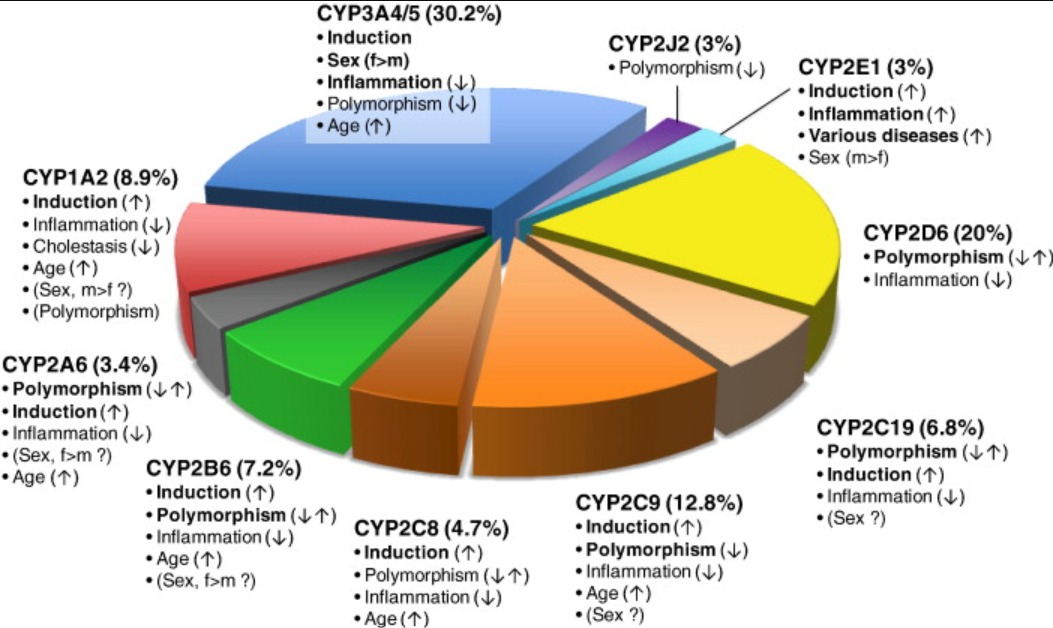
\includegraphics[width=0.7\textwidth]{img/grafica_cyp.jpeg} 
    \caption{Regulación de la expresión génica y actividades enzimáticas del CYP (fuente: \cite{zanger2013cytochrome}).}
    \label{fig:grafica_cyp}
\end{figure}

\subsection{Inducción e inhibición enzimática}
Las enzimas del sistema CYP450 pueden verse afectadas por la presencia de determinados fármacos o sustancias externas.

La inducción enzimática consiste en un aumento de la actividad metabólica de una enzima, lo que provoca una eliminación más rápida de los medicamentos metabolizados por dicha vía y, en consecuencia, una posible disminución de su efecto terapéutico.

Por el contrario, la inhibición enzimática reduce la actividad de la enzima, aumentando las concentraciones plasmáticas del fármaco afectado y el riesgo de aparición de efectos adversos o toxicidad.

Estos fenómenos constituyen uno de los principales mecanismos responsables de las interacciones farmacológicas de tipo farmacocinético.

Debido a que numerosos medicamentos comparten las mismas vías metabólicas, el sistema CYP450 constituye uno de los principales responsables de las interacciones fármaco-fármaco. Cuando dos o más fármacos son administrados simultáneamente, pueden competir por una misma enzima, inducir su actividad o inhibirla, alterando las concentraciones plasmáticas de alguno de ellos.


\section{Sistema de Clasificación Anatómica, Terapéutica y Química (ATC)}
El Sistema ATC es un estándar internacional de codificación de sustancias farmacéuticas y medicamentos \cite{whocc_home}. Instaurado y mantenido por el Centro Colaborador de la Organización Mundial de la Salud (OMS) para la Metodología de Estadísticas sobre medicamentos.
Este sistema constituye una herramienta fundamental en la informática biomédica para la interoperabilidad de datos clínicos, la farmacovigilancia y el análisis epidemiológico \cite{who_atc_classification}.

El objetivo principal del sistema ATC es servir como un instrumento estandarizado para la presentación de estadísticas sobre el consumo de medicamentos a nivel global, permitiendo la comparación armonizada de datos entre diferentes regiones, centros hospitalarios y periodos de tiempo \cite{who_atc_methodology}.

A cada fármaco le corresponde un único código ATC que lo clasifica según su principal indicación terapéutica. Los principio activos contenidos en los fármacos pueden tener más de un código ATC, en el caso en el que éste se emplee en indicaciones o en formas farmacéuticas diferentes, sin embargo, no hay un mismo código ATC completo asociado a mas de un principio activo\cite{sacyl_uso_racional}

\subsection{Estructura y Jerarquía del Código ATC}
El sistema ATC se organiza de forma jerárquica en cinco niveles independientes. Cada principio activo recibe un código alfanumérico único de 7 caracteres que detalla desde el sistema orgánico sobre el que actúa hasta su estructura química específica \cite{whocc_structure} .

La arquitectura de dichos niveles se estructura de la siguiente manera  \cite{whocc_structure} \cite{who_atc_classification} :
\begin{enumerate}
    \item \textbf{Nivel Anatómico.} Consta de una letra que indica el grupo anatómico principal, es decir, el órgano o sistema sobre el que actúa el fármaco (en total existen 14 grupos principales).
    \item \textbf{Nivel Terapéutico} Formado por un código numérico de dos dígitos que identifica el grupo terapéutico principal.
    \item \textbf{Nivel Farmacológico/Terapéutico.} Constituido por una letra que especifica el subgrupo terapéutico o farmacológico.
    \item \textbf{Nivel Químico.} Compuesto por una letra que define el subgrupo químico, terapéutico o farmacológico detallado.
    \item \textbf{Nivel Sustancia Química.} Formado por un código numérico de dos dígitos que designa de manera exclusiva la sustancia química o principio activo individual.
\end{enumerate}


\section{Herramientas para la Base de Datos y la visualización}
Para la generación de los conjuntos de datos consolidados \texttt{DDI\_sea.csv} y \texttt{efectos\_adversos.csv}, se ha extraído e integrado la información procedente de las plataformas de referencia internacional DrugBank \cite{drugbank}, SIDER \cite{sider} y el portal oficial CIMA \cite{cima}. 

Por otro lado, la visualización de los resultados y el análisis de las interacciones farmacológicas se ha implementado mediante el entorno de desarrollo Dash \cite{dash_framework}. Este enfoque permite desplegar un cuadro de mando interactivo que facilita la interpretación de las interacciones y sus causas etiológicas por parte del personal facultativo de manera intuitiva.

A continuación, se detallan las características y el propósito analítico de cada una de las herramientas seleccionadas

\subsection*{DrugBank}
DrugBank es una base de datos biológica y bioinformática de acceso público y gratuito para fines académicos que centraliza información sumamente detallada sobre medicamentos y sus dianas terapéuticas.
En este proyecto, se ha utilizado para recuperar los nombres de los principios activos y sus correspondientes códigos ATC. Asimismo, permite identificar las enzimas metabólicas asociadas, las dianas biológicas hacia las que se dirigen los compuestos y sus respectivos mecanismos de acción.

\subsection*{CIMA}
CIMA son las siglas del Centro de Información Online de Medicamentos de la Agencia Española de Medicamentos y Productos Sanitarios (AEMPS). Es una base de datos pública, oficial y gratuita que contiene todos los medicamentos autorizados en España, así como aquellos cuya autorización ha sido revocada, suspendida o caducada.
En el marco de este trabajo, se han aplicado técnicas de extracción automatizada de datos (web scraping) sobre sus fichas técnicas oficiales. El objetivo principal de este proceso es resolver ambigüedades en aquellos principios activos para los que DrugBank identifica múltiples vías metabólicas, logrando así determinar con precisión cuál es la enzima principal responsable de su metabolismo.

\subsection*{SIDER}
SIDER es una base de datos bioinformática de acceso público cuyo propósito principal es centralizar, registrar y conectar información estructurada sobre los efectos secundarios de los medicamentos y sus frecuencias de aparición clínicamente documentadas por mas de una fuente. Sirve como un recurso complementario a plataformas como DrugBank.
Esta plataforma se ha empleado de forma complementaria para asociar a cada principio activo su perfil de efectos secundarios y la probabilidad de manifestación de los mismos. Ademas, integra la codificación estandarizada ATC para cada sustancia, lo que facilita la recuperación de su información.

\subsection*{DASH}
El entorno de desarrollo de DASH tiene la capacidad de transformar almacenes de datos biomédicos complejos en interfaces analíticas comprensibles para la visualización de los resultados. Se ha consolidado como un framework de código abierto fundamental para la construcción de aplicaciones web analíticas e interactivas utilizando exclusivamente lenguajes de programación científicos como Python, R o Julia.


\section{Estado del arte y trabajos relacionados.}
En los últimos años se han desarrollado numerosas herramientas destinadas a detectar posibles interacciones entre medicamentos (Drug-Drug Interactions, DDI), tanto en el ámbito investigador como en aplicaciones de uso clínico. La mayoría de estas soluciones permiten consultar la posible interacción entre dos o más principios activos, proporcionando un nivel de gravedad junto con recomendaciones clínicas. Sin embargo, pocas ofrecen una explicación detallada del mecanismo farmacocinético responsable de la interacción o permiten explorar alternativas terapéuticas de forma integrada.

Uno de los trabajos académicos mas relevantes es el publicado en 2024 en PubMed \cite{pubmed_39180399}, donde se presenta un sistema basado en información farmacológica para el estudio de interacciones entre fármacos. El trabajo pone de manifiesto la importancia de integrar bases de datos biomédicas y mecanismos moleculares para mejorar la interpretación de las interacciones de medicamentos. 

En el ámbito de las bases de datos especializadas destaca DDInter2 \cite{ddinter_database}, una plataforma que recopila información procedente de diferentes fuentes bibliográficas y bases de datos farmacológicas. Esta herramienta ofrece una gran cobertura de interacciones conocidas, indicando el mecanismo implicado, el nivel de evidencia y referencias bibliográficas. Su principal fortaleza reside en la amplitud de la información disponible, aunque la cantidad de datos mostrados puede dificultar la interpretación rápida por parte de usuarios no especializados.

Entre las herramientas de uso clínico más extendidas se encuentran los comprobadores de interacciones de Medscape \cite{medscape_checker}, RxList \cite{rxlist_checker} y Drugs.com \cite{drugs_checker}. Estas plataformas permiten consultar rápidamente posibles interacciones entre medicamentos y clasificarlas según su gravedad clínica. Además, suelen incorporar recomendaciones generales para el profesional sanitario. Sin embargo, su funcionamiento se basa principalmente en mostrar el resultado de la interacción y una descripción textual, sin explicar de manera detallada el razonamiento seguido para alcanzar dicha clasificación.

La herramienta desarrollada en este Trabajo Fin de Grado adopta un enfoque diferente al de las soluciones existentes. En lugar de limitarse a indicar si existe o no una interacción, analiza el metabolismo de ambos principios activos utilizando la información contenida en DrugBank sobre enzimas metabolizadoras, prestando especial atención a las enzimas CYP más relevantes (CYP3A4, CYP3A5, CYP2D6, CYP2C9, CYP2C19 y CYP1A2). A partir de esta información determina un nivel de riesgo (bajo, medio o alto) en función de la coincidencia de las enzimas implicadas y de si estas han sido identificadas como principales en el metabolismo de cada fármaco.

Además de clasificar el riesgo, proporciona una explicación del motivo de la interacción, indicando las enzimas compartidas y el papel que desempeña cada principio activo sobre ellas (sustrato, inhibidor o inductor). Esta característica aporta un componente de interpretabilidad que no suele encontrarse en los comprobadores comerciales, permitiendo comprender el mecanismo farmacocinético responsable de la posible interacción.

Otra contribución diferencial consiste en la incorporación de un módulo de búsqueda de alternativas terapéuticas basado en la clasificación ATC. Cuando se detecta una interacción de riesgo medio o alto, el sistema identifica principios activos pertenecientes al mismo grupo terapéutico y evalúa automáticamente todas las combinaciones posibles hasta encontrar aquellas cuya interacción se clasifica como de bajo riesgo. De esta forma, la herramienta no solo identifica el problema, sino que propone posibles soluciones consideradas seguras para el algoritmo.

Finalmente, la aplicación integra información sobre efectos adversos procedente de la base de datos SIDER, mostrando gráficamente los efectos secundarios más frecuentes asociados a los códigos ATC de referencia. Esta funcionalidad proporciona información adicional que puede resultar útil durante la valoración de posibles alternativas terapéuticas.

\capitulo{4}{Metodología}

\setsecnumdepth{subsubsection}

\section{Descripción de los datos}
En este apartado se detalla la información obtenida de las tres bases de datos públicas de referencia utilizadas en este proyecto: DrugBank \cite{drugbank}, SIDER \cite{sider} y CIMA \cite{cima}.

Además se especifican los criterios de selección y filtrado de datos para la realización de los conjuntos de datos creados.
\paragraph{SIDER}
Se descargaron los registros estructurados en formato TSV correspondientes a efectos adversos (\texttt{meddra\_all\_se.tsv}), frecuencias de aparición (\texttt{meddra\_freq.tsv}) y mapeo de nombres (\texttt{drug\_names.tsv}). A través de un cruce indexado por identificador de compuesto (flat), se unificó la información para calcular la frecuencia media de aparición de cada síntoma recogido en el documento llamado \texttt{efectos\_adversos.csv}.
Mas tarde se incluye a el documento mencionado una columna adiccional con los códigos ATC únicos de cada principio activo obtenidos del documento llamado \texttt{drug\_atc.tsv} para poder facilitar la interoperabilidad con las siguientes bases de datos consultadas y el fácil acceso por parte de la herramienta generada.

\paragraph{DrugBank}
Se utilizó como la ontología central para el modelado de fármacos, dianas y rutas metabólicas. La adquisición se realizó mediante la descarga de su base de datos completa en formato XML (\texttt{full\_database.xml}), procesando mediante parsing un total de 10.162 principios activos únicos. De este repositorio se extrajeron de forma dirigida los campos de identificador binario (\texttt{drugbank\_id}), nombre genérico, sinónimos comerciales, tipos de interacción (diana o enzima), nombre del gen codificante y acciones farmacodinámicas asociadas.

\paragraph{CIMA}
Se extrajo e iteró la base de datos estructurada de prescripción (Prescripcion.xml) junto a sus diccionarios auxiliares de formas farmacéuticas y situaciones de registro. Esto permitió trabajar con 30.232 registros de medicamentos autorizados en España. De las cuales, como se explica mas adelante se intentarán obtener las fichas técnicas de 665 registros concretos.

\subsection{Criterio inclusión/exclusión}
Para acotar el alcance del proyecto se aplicaron de forma secuencial los siguientes criterios de selección (filtros de inclusión/exclusión):
\begin{itemize}
    \item \textbf{Restricción del Perfil Enzimático (Top 6 CYP).} Tras analizar la distribución de frecuencias de las enzimas en DrugBank, se constató que la familia del citocromo P450 concentraba la inmensa mayoría de las rutas metabólicas de fase I. Se acotó el diseño computacional a las seis isoenzimas con mayor impacto y frecuencia de aparición (visible en la tabla \ref{fig:frecuencia_cyp} creada en un notebook auxiliar no incluido): CYP3A4, CYP2C9, CYP2D6, CYP1A2, CYP2C19 y CYP3A5. Se incluyó CYP3A5 debido a su estrecha relación con CYP3A4. 
    \item \textbf{Criterio Base de Datos de CIMA.} De estos registros inicialmente extraídos se excluyeron los medicamentos compuestos por mas de un principio activo. Esto permitió aislar 25.453 medicamentos monofármaco. De estos, eliminando duplicidades de presentaciones comerciales, se identificaron 2.100 principios activos puros validados para el mercado español.
    \item \textbf{Filtrado Ontológico de Efectos Adversos.} Por último para el procesamiento de SIDER, se aplicó un criterio de exclusión sobre la columna \texttt{meddra\_type}, descartando los términos generales (LLT) y limitando la Ingesta únicamente a los Términos Preferidos (PT, Preferred Terms). Esto redujo el conjunto final a 968 compuestos químicos con perfiles de toxicidad normalizados y frecuencias cuantitativas verificadas.
\end{itemize}

\begin{figure}[h]
    \centering
    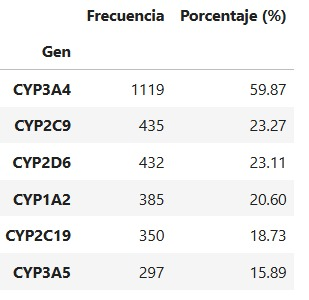
\includegraphics[width=0.35\textwidth]{img/frecuencias_cyp.jpeg} 
    \caption{Resumen frecuencia de aparición de las enzimas seleccionadas en DrugBank}
    \label{fig:frecuencia_cyp}
\end{figure}

\subsection{Criterio de resolución de ambiguedades}
Cuando un principio activo presentaba múltiples enzimas del citocromo P450 seleccionadas en DrugBank de forma simultánea, el sistema informático se encontraba ante una ambigüedad matemática para determinar el riesgo de interacción asociado. Por tanto, se intentará detectar la via metabólica principal que sigue cada uno de los 753 principios activos en los que esto sucede.

Para ello se filtran tan solo los que tienen como acción sustrato \footnote{sustrato: que posean como acción sustrato significa que la enzima actúa de manera directa sobre una molécula específica para transformarla químicamente \cite{biolan_health_enzimas}}, lo que reduce el conjunto a 665 registros, después, se seleccionaron de forma programática los códigos ATC coincidentes entre DrugBank y CIMA de esos principios activos, lo que nos reduce un más el conjunto de datos a 418 registros. Sobre estos se ejecutó un algoritmo de extracción (mediante web scraping \footnote{Web scrapping: técnica que se utilizada para extraer información de sitios web de manera automatizada \cite{esic_web_scraping}.}) sobre sus respectivas fichas técnicas oficiales. En el presente proyecto primero se descargaron de manera programática cada uno de los pdfs correspondientes a las fichas técnicas (en caso de encontrarse) de cada principio activo problema (en un periodo prolongado de tiempo, evitando de esta manera errores del tipo 429 \footnote{error 429: too many requests, significa que el servidor rechaza temporalmente la conexión por saturación de tráfico (muchas solicitudes en poco tiempo).}). 

Esta información textual extraída fue procesada mediante modelos de lenguaje vectorizados (NotebookLM y ChatGPT) para determinar cuál de las enzimas registradas ejercía el rol de vía metabólica principal (categorizada como prioridad = 1) frente a las secundarias y su posterior creación de un dataframe con esta información con el objetivo de poder incluirlo con los datos extraídos de DrugBank. Cuando no fue posible encontrar ninguna via principal se categorizan a todas las presentes en ese principio activo como prioridad = 0.

Debido a las limitaciones temporales y al elevado volumen de documentación bibliográfica por analizar, se optó por el uso de herramientas de Inteligencia Artificial (IA) para la identificación de la enzima principal. En concreto, se seleccionó NotebookLM para la revisión de las fichas técnicas, dado que este modelo opera exclusivamente con las fuentes de información suministradas por el usuario (con un límite de 50 documentos por consulta), lo que minimiza el riesgo de alucinaciones.

El procedimiento consistió en la introducción secuencial de bloques de registros previamente segmentados. A partir de estos datos, se consultó al modelo sobre la presencia de la enzima principal para cada fármaco; en caso de ausencia de resultados, se parametrizó la respuesta para devolver el valor None. Finalmente, con el objetivo de optimizar el procesamiento de datos y evitar la transcripción manual, se empleó ChatGPT para la estructuración y conversión de los resultados obtenidos en un dataframe(df) \footnote{dataframe (df): estructura de datos que los organiza en una tabla bidimensional de filas y columnas, similar a un excel}. 

Posteriormente, se filtró el dataframe mediante la exclusión de aquellos fármacos cuya enzima principal no coincidía con las seleccionadas para el presente proyecto. Asimismo, en los casos donde se identificaron simultáneamente las enzimas CYP3A4 y CYP3A5 como principales, se optó por descartar esta última. Dicha decisión se fundamenta en que, debido a la alta prevalencia de polimorfismos genéticos asociados a CYP3A5, la mayoría de la población humana no expresa de forma funcional esta isoenzima.

\section{Técnicas y herramientas.}
Para el desarrollo del sistema de detección e interpretación de interacciones farmacológicas, se ha diseñado un flujo de trabajo enfocado en la ingeniería de datos biomédicos, el procesamiento de lenguaje natural y la visualización analítica. A continuación, se detallan las técnicas e infraestructuras de software implementadas:

\subsection{Entorno de Programación y Librerías Científicas}
La extracción y procesamiento de los datos y la lógica computacional, se han implemantado bajo el lenguaje de programación Python. Para la manipulación y estructuración matricial de la información se ha utilizado la librería de código abierto Pandas, permitiendo realizar operaciones complejas de unificación (merge), filtrado por condiciones y agregación de variables bioinformáticas. Asimismo, se ha empleado la biblioteca nativa ElementTree (ET) para la lectura y extracción eficiente en términos de memoria de archivos extensos estructurados en formato XML.

\subsection{Técnicas de Extracción y Consolidación de Datos}
Debido a la heterogeneidad y procedencia de las fuentes originales, ha sido necesario aplicar diferentes técnicas de ingeniería de datos para unificar los identificadores de los principios activos y posibilitar la interoperabilidad entre las diferentes fuentes:

\begin{itemize}
    \item \textbf{Estandarización de Identificadores mediante Código ATC.} Para resolver las discrepancias nomenclátricas entre las bases de datos americanas, europeas y nacionales, se ha utilizado el sistema de clasificación jerárquica de la Organización Mundial de la Salud (OMS). Los códigos ATC se han empleado como clave primaria universal para cruzar e integrar registros procedentes de plataformas inicialmente inconexas.
    \item \textbf{Procesamiento de Estructuras Jerárquicas Complejas.} Dado que un único fármaco puede presentar múltiples acciones biológicas o códigos de indexación anatómica, se ha utilizado la técnica de explosión de colecciones en filas (exploding) sobre vectores previamente divididos. Esto ha permitido aislar cada tupla "principio activo - acción"  o "principio activo - código ATC"  de manera simplificada para evitar sesgos en el análisis posterior.
    \item \textbf{Técnicas de Web Scraping y Peticiones Programáticas Controladas.} La recopilación de las fichas técnicas oficiales de CIMA se ha realizado de forma automatizada mediante la biblioteca Requests. Para evitar sobrecargar los servidores gubernamentales de la AEMPS y prevenir la aparición de errores del tipo 429, por tanto, la columna llamada 'Prioridad' en el documento \texttt{DDI\_sea.csv} se ha implementado de forma asíncrona segmentando el volumen total (418) en bloques reducidos de 40 registros e introduciendo retrasos controlados en la ejecución.
\end{itemize}



\section{Metodología de Ingeniería del Software}
En esta sección se detalla el marco metodológico, el conjunto de tecnologías y el flujo de arquitectura de software implementados para el desarrollo, despliegue y puesta en producción de la interfaz interactiva del presente proyecto.

\subsection*{Framework de visualización: Dash}
Para la construcción de la interfaz interactiva y la representación de los datos analizados, se seleccionó el entorno de desarrollo \textit{Plotly Dash}. Dash es un framework de código abierto basado en Python, lo que simplifica significativamente su programación al omitir la necesidad de requerir conocimientos avanzados en desarrollo \textit{frontend} \footnote{Desarrollo frontend: subárea de la ingeniería de software enfocada en el diseño, estructura y creación de la interfaz visual de un sitio web o aplicación con la que interactúa el usuario.}.

La elección de esta herramienta frente a otras alternativas se fundamentó en su capacidad para diseñar soluciones ágiles. A diferencia de las plataformas comerciales o herramientas ya existentes para la consulta de interacciones farmacológicas (las cuales suelen integrar volúmenes masivos de información que pueden saturar la toma de decisiones del facultativo), uno de los objetivos de este proyecto requería una arquitectura visualmente eficiente. De este modo, Dash permitió estructurar un cuadro de mando donde, el profesional sanitario puede identificar los datos críticos esenciales, incluyendo la información ampliada bajo demanda y las alternativas farmacológicas consideradas seguras.

\subsection*{Renderización de la visualización: Render}
Una vez completado el desarrollo local de la interfaz interactiva, se procedió a su despliegue en un entorno de producción a través de la plataforma Render \cite{render}. La selección de esta infraestructura frente a otras alternativas se justificó por su alto grado de automatización y su capacidad de integración continua con repositorios de control de versiones. Esto permitió agilizar los tiempos de computación, garantizando la disponibilidad inmediata y estable de la aplicación web de cara a la fase de evaluación y defensa ante el tribunal examinador.




\capitulo{5}{Resultados}
Los resultados obtenidos en este Trabajo de Fin de Grado muestran la viabilidad de desarrollar una herramienta capaz de integrar información farmacológica procedente de distintas bases de datos heterogéneas con el objetivo de detectar posibles interacciones entre principios activos.

\section{Funcionamiento de la interfaz}
En relación con el objetivo general, se ha logrado implementar un sistema funcional que permite analizar la interacción entre fármacos a partir de las enzimas implicadas en su metabolismo. La herramienta desarrollada proporciona una visualización clara de los resultados, facilitando de esta manera la interpretación por parte del usuario final.

Todos los ejemplos mostrados en los siguientes resultados son para la interacción clopidogrel-omeprazole. Además, todas las explicaciones se encuentran en inglés debido a que, de esta manera, la aplicación podrá ser utilizada por cualquier persona.

Una vez dentro de la plataforma se encuentra la interfaz principal \ref{fig:pag_ppal} que posee un logo creado en la parte superior, una breve descripción de la funcionalidad de la herramienta y las enzimas tenidas en cuenta para la interacción junto a un menú lateral con las diferentes pestañas en las que introduciremos cada uno de los principios activos. 
\begin{figure}[h]
    \centering
    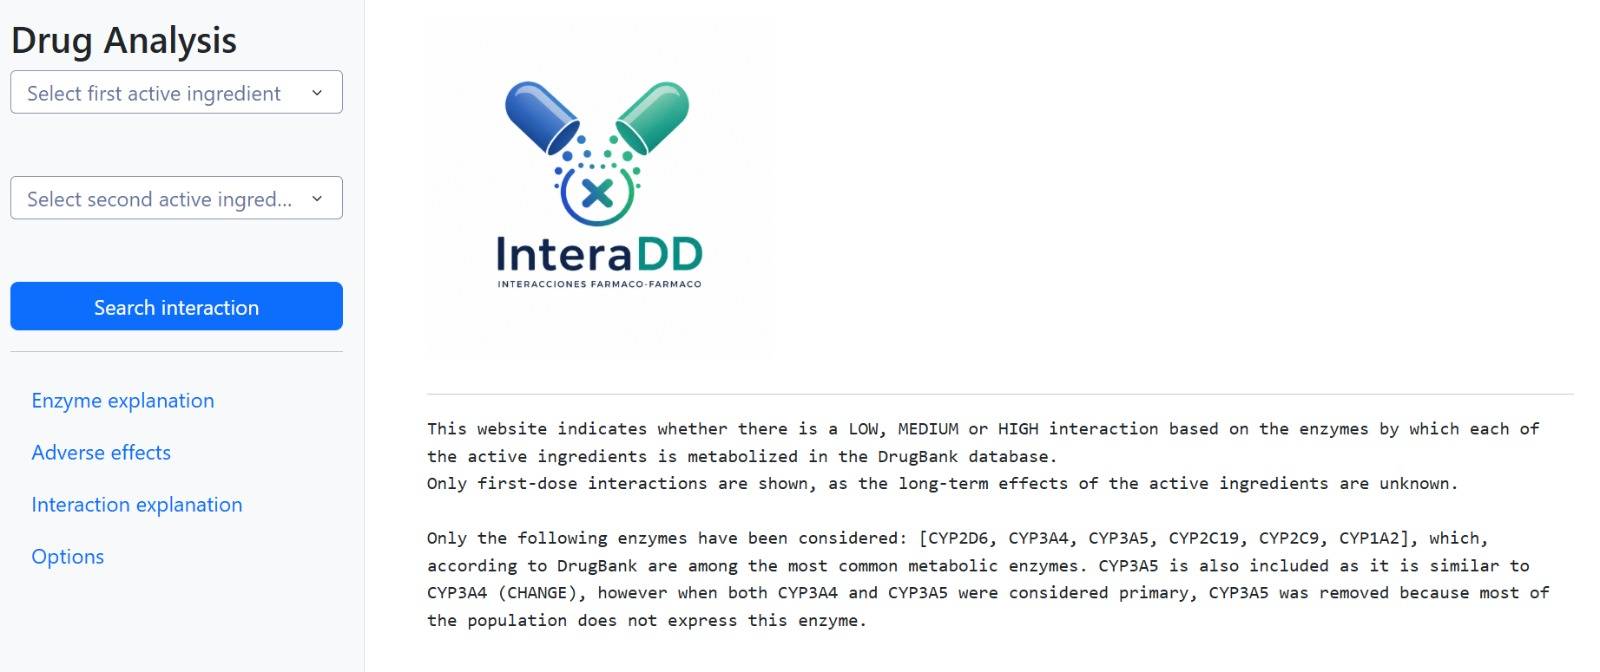
\includegraphics[width=0.5\textwidth]{img/pagina_principal.jpeg} 
    \caption{Página principal de la herramienta desarrollada}
    \label{fig:pag_ppal}
\end{figure}

Tras introducir los pares de principios activios y pulsar el boton de “search interaction” nos aparece el nivel de interacción en un cuadro de texto codificado por colores (rojo/amarillo/verde) y en caso necesario de saber el porque de dicho nivel, hay un desplegablee con la correspondiente explicación visible en la siguiente imagen \ref{fig:buscar_interaccion}. Esta información nunca se elimina de la interfaz visual hasta el momento en el que se busca otra interacción diferente con otros principios activos distintos. 

\begin{figure}[h]
    \centering
    
\includegraphics[width=0.5\textwidth]{img/interaccion.jpeg} 
    \caption{Cuadro fijo}
    \label{fig:buscar_interaccion}
\end{figure}

Por otro lado, el botón "enzyme explanation" nos ofrece las enzimas principales de los principios activos solicitados, en caso de tenerlas, y una breve explicación del criterio de selección de dichas enzimas, un ejemplo del mismo es el visto en la siguiente imagen \ref{fig:enzimas}.

\begin{figure}[h]
    \centering
    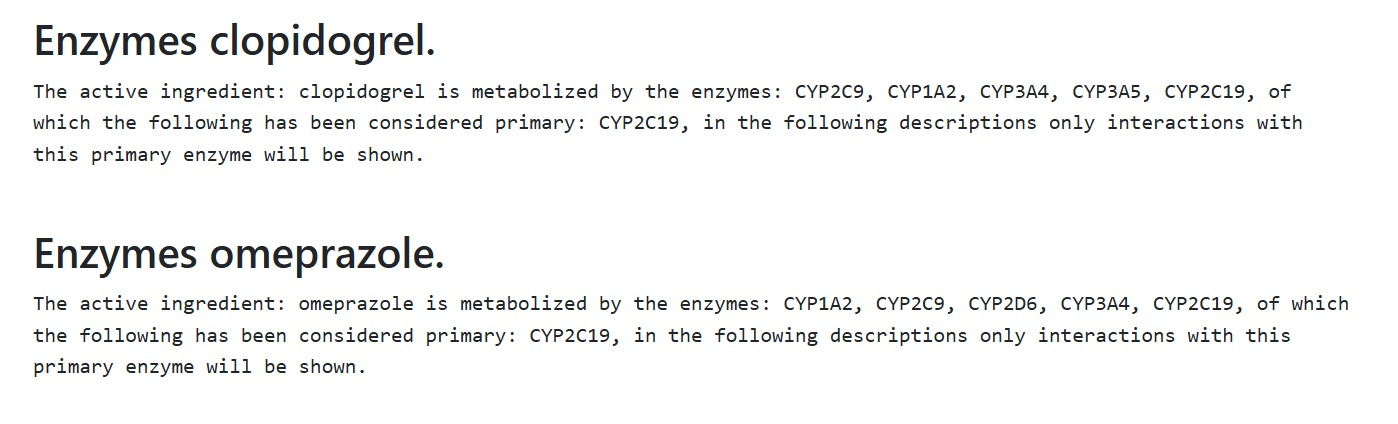
\includegraphics[width=0.5\textwidth]{img/exp_enz.jpeg} 
    \caption{Explicación de enzimas}
    \label{fig:enzimas}
\end{figure}

En el módulo de efectos adversos, nos muestra en un gráfico de barras interactivo, los principales efectos adversos según el/los código/s ATC de referencia de cada principio activo introducido, se puede ver en la imagen adjunta \ref{fig:grafico_ea}.

\begin{figure}[h]
    \centering
    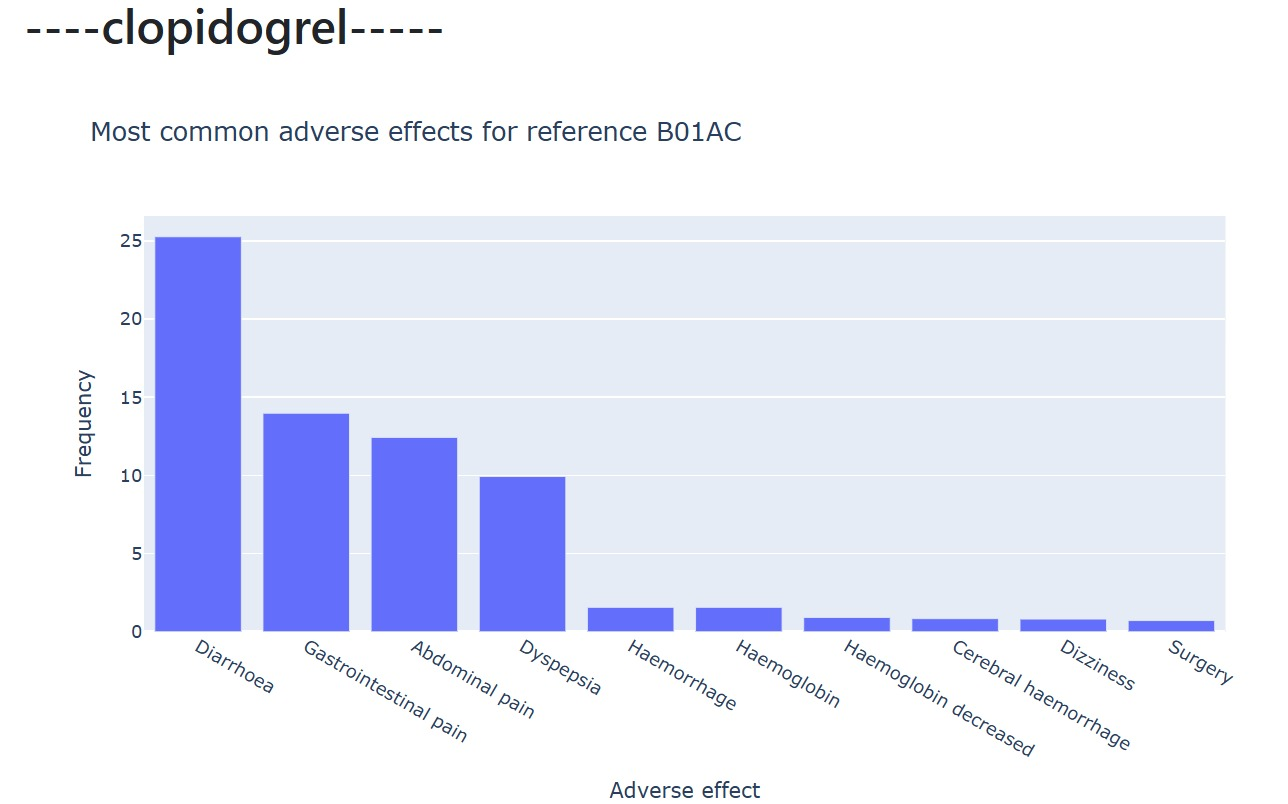
\includegraphics[width=0.5\textwidth]{img/diagrama_ea.jpeg} 
    \caption{Diagrama de barras de efectos adversos}
    \label{fig:grafico_ea}
\end{figure}

Otro de los botones incluidos "Interaction explanation" explica el mecanismo de acción que siguen ambos principios para las enzimas detectadas por el algoritmo como coincidentes, indicando de esta manera el nivel de prevalencia de una sobre otra, se puede observar en la siguiente imagen \ref{fig:acciones}.

\begin{figure}[h]
    \centering
    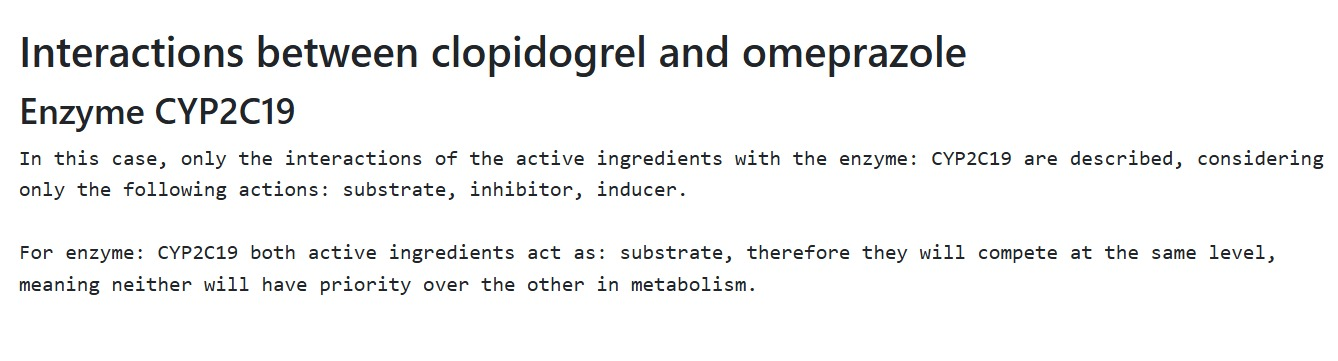
\includegraphics[width=0.5\textwidth]{img/exp_acciones.jpeg} 
    \caption{Explicación de las acciones de cada enzima que hace que los principios interactúen.}
    \label{fig:acciones}
\end{figure}

Finalmente, en la pestaña "options" podemos ver alternativas terapéuticas consideradas seguras para el algoritmo, en caso de que la interacción entre los principios activos resulte ser media-alta, se muestran las alternativas para los principios activos seleccionados en la imagen \ref{fig:alternativas}.

\begin{figure}[h]
    \centering
    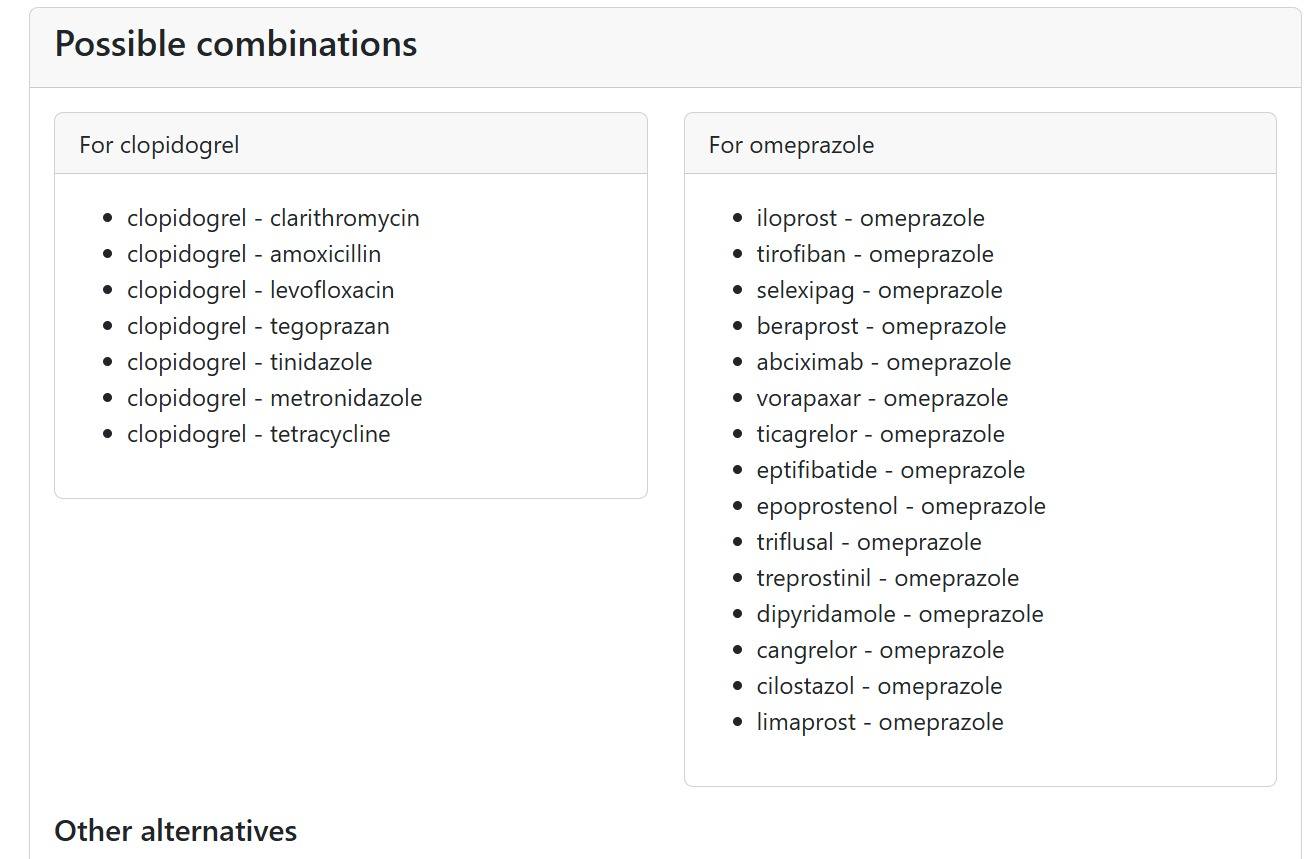
\includegraphics[width=0.5\textwidth]{img/opciones.jpeg} 
    \caption{Posibles alternativas terapéuticas clopidogrel-omeprazole.}
    \label{fig:alternativas}
\end{figure}

En conjunto, el sistema desarrollado cumple los objetivos planteados, proporcionando una herramienta funcional para el análisis de interacciones farmacológicas y proposición de alternativas seguras. No obstante, su uso debe entenderse como un sistema de apoyo a la decisión y no como una herramienta clínica definitiva.

\section{Casos de prueba}

PRIMERO TENGO QUE SOLUCIONAR EL RENDER
\capitulo{6}{Discusión}

\section{Discusión de los resultados}
El desarrollo de la herramienta informática presentada en este trabajo demuestra la viabilidad técnica y metodológica de integrar fuentes de datos biomédicos heterogéneas (DrugBank, CIMA y SIDER) para construir un sistema interpretable de detección de interacciones farmacológicas (DDI \footnote{DDI: drug-drug interaction}) basado en el metabolismo de las enzimas CYP3A4, CYP3A5, CYP2D6, CYP2C9, CYP2C19 y CYP1A2. 
A diferencia de las soluciones comerciales dominantes mencionadas en el apartado de estado del arte esta herramienta desarrollada adopta un enfoque donde en lugar de limitarse a indicar si existe o no una interacción, analiza el metabolismo de ambos principios activos utilizando la información contenida en DrugBank sobre enzimas metabolizadoras, prestando especial atención a las enzimas CYP más relevantes. A partir de esta información determina un nivel de riesgo (bajo, medio o alto) en función de la coincidencia de las enzimas implicadas y de si estas han sido identificadas como principales en el metabolismo de cada fármaco.

Además de clasificar el riesgo, proporciona una explicación del motivo de la interacción, indicando las enzimas compartidas y el papel que desempeña cada principio activo sobre ellas (sustrato, inhibidor o inductor). Esta característica aporta un componente de interpretabilidad que no suele encontrarse en los comprobadores comerciales, permitiendo comprender el mecanismo farmacocinético responsable de la posible interacción.

Otra contribución diferencial consiste en la incorporación de un módulo de búsqueda de alternativas terapéuticas basado en la clasificación ATC. Cuando se detecta una interacción de riesgo medio o alto, el sistema identifica principios activos pertenecientes al mismo grupo terapéutico y evalúa automáticamente todas las combinaciones posibles hasta encontrar aquellas cuya interacción se clasifica como de bajo riesgo. De esta forma, la herramienta no solo identifica el problema, sino que propone posibles soluciones consideradas seguras para el algoritmo.

Finalmente, la aplicación integra información sobre efectos adversos procedente de la base de datos SIDER, mostrando gráficamente los efectos secundarios más frecuentes asociados a los códigos ATC de referencia. Esta funcionalidad proporciona información adicional que puede resultar útil durante la valoración de posibles alternativas terapéuticas.

Los resultados obtenidos en general son los esperados para los ejemplos comprobados explicados en el apartado de 
resultados, a excepción de las explicaciones de las acciones implicadas. Por lo tanto, con el presente proyecto se han logrado implementar 
las nuevas funcionalidades de propuesta de alternativas terapéuticas y explicación de las enzimas implicadas en la interacción que no encontramos presentes herramientas comerciales existentes.

Uno de los mayores desafíos abordados en este proyecto ha sido la resolución de ambigüedades en fármacos con perfiles metabólicos múltiples. Mientras que plataformas como DrugBank listan de manera exhaustiva todas las enzimas con las que un principio activo puede interactuar, carecen en muchos casos de una jerarquización cuantitativa o clínica de estas vías. La estrategia metodológica de realizar un \textit{web scraping} dirigido sobre las fichas técnicas de la AEMPS a través de CIMA, complementado con el procesamiento mediante modelos de NotebookLM y ChatGPT, ha permitido discriminar de forma efectiva las vías metabólicas principales (Prioridad = 1) de las secundarias. 

Por otra parte, el producto desarrollado en el presente proyecto debe considerarse como una prueba de concepto incial debido a una serie de limitaciones:
\begin{itemize}
    \item \textbf{Incertidumbre en la determinación de las vías metabólicas principales:} La dificultad para identificar inequívocamente la ruta metabólica predominante de ciertos principios activos puede derivar en una estimación menor del nivel de gravedad de las interacciones. Esto podría provocar que interacciones clínicamente significativas se categoricen erróneamente como medias o leves, debido a la posible equivocación de la asignación de la isoenzima primaria en la base de conocimiento creada.
    
    \item \textbf{Sesgo de simplificación por selección acotada de isoenzimas:} Al restringir la base de datos creada a las isoenzimas más importantes del sistema CYP450, se asume una simplificación que afecta a fármacos con perfiles metabólicos complejos o rutas alternativas. Consecuentemente, existe el riesgo de clasificar como leve una interacción cuyo aclaramiento dependa mayoritariamente de enzimas excluidas del análisis, limitando el registro a la identificación de dianas moleculares sin su correspondiente correlación enzimática.
    
    \item \textbf{Dependencia de la calidad y completitud de repositorios públicos:} El rendimiento del sistema está estrictamente supeditado a la integridad de las bases de datos externas consultadas. Se ha detectado la presencia de valores nulos (\textit{missing values}) en campos críticos para la interoperabilidad del sistema, tales como los códigos del sistema de Clasificación Anatómica, Terapéutica y Química (ATC) o el mecanismo de acción específico (inducción/inhibición) de las isoenzimas.
    
    \item \textbf{Limitaciones en el procesamiento de lenguaje natural (PLN) sobre textos no estructurados:} La extracción automatizada de información a partir de fuentes de texto libre, como las fichas técnicas de la Agencia Española de Medicamentos y Productos Sanitarios (CIMA), presenta restricciones operativas. La ambigüedad de los textos médicos no estructurados dificulta la validación exhaustiva de aquellos registros donde la Inteligencia Artificial identifica múltiples enzimas metabólicas concurrentes para un mismo fármaco.
\end{itemize}




\capitulo{7}{Conclusiones}

\section{Conclusiones sobre los resultados del proyecto}
El desarrollo de este Trabajo Fin de Grado ha permitido alcanzar con éxito el objetivo general y cada uno de los objetivos específicos planteados originalmente. Las principales conclusiones derivadas de los resultados obtenidos son las siguientes:

\begin{itemize}
    \item \textbf{Viabilidad de la detección de interacciones.} Se ha demostrado que es posible automatizar la detección de interacciones farmacológicas y dotar al sistema de un componente de interpretabilidad clínica analizando las isoenzimas del sistema CYP450, superando el modelo clásico de las plataformas comerciales a la hora de mostrar la información de manera más sencilla.
    \item \textbf{Efectividad del módulo de alternativas:} El algoritmo basado en la jerarquía de códigos ATC ha probado ser una solución robusta para resolver interacciones de riesgo medio y alto, identificando de esta manera con precisión principios activos equivalentes terapéuticamente pero con rutas metabólicas compatibles, por las cuales no se detecte interacción.
    \item \textbf{Utilidad del cuadro de mando integrado:} La interfaz web interactiva centraliza de manera eficiente tres flujos de información críticos para el personal facultativo (el nivel de riesgo, el porqué biológico de la interacción y el perfil de toxicidad de SIDER). El diseño de esta herramienta permite al usuario visualizar de manera eficaz la información necesaria para modificar algún principio activo de los recetados en caso de ser necesario.
    \item \textbf{Interoperabilidad de fuentes heterogéneas:} El uso del código ATC de la OMS como clave primaria universal ha demostrado ser la estrategia idónea para unificar las estructuras de datos consultadas como fichas técnicas en formato PDF (CIMA), bases de datos en XML (DrugBank) y registros estructurados en TSV (SIDER).
    \item \textbf{Eficiencia de arquitecturas ligeras:} La arquitectura integrada por Python, Pandas, Plotly Dash y el despliegue en Render confirma que es posible construir interfaces analíticas de alto rendimiento y producción estable para el sector farmacéutico sin necesidad de complejas herramientas usadas tradicionalmente.
\end{itemize}

\section{Aspectos relevantes.}
Durante el desarrollo del presente software, se han tomado decisiones arquitectónicas y metodológicas clave que transformaron el enfoque del proyecto:

\subsection*{El fracaso de la aproximación por fuerza bruta en DrugBank (Resultados negativos)}
En las primeras fases del diseño del algoritmo de detección de interacciones, se intentó operar exclusivamente con los datos de DrugBank. El planteamiento inicial consistía en mostrar las interacciones basándose  en su vía de metabolización. Este enfoque supuso un problema debido a la gran cantidad de principios activos con perfiles metabólicos múltiples existentes en la misma,  cuando se planteó la idea de no proponer vía metabólica principal surgió un problema: habría interacciones que se categorizaran como altas o medias cuando deberían ser leves.

Este obstáculo obligó a pivotar el diseño hacia la introducción de un parámetro de prioridad. Entender que necesitábamos discriminar de forma matemática qué enzima era la vía principal frente a las vías secundarias fue el punto de inflexión del proyecto y lo que motivó la inclusión de CIMA en el desarrollo del mismo.

\subsection*{Justificación del Web Scraping asíncrono y control de errores 429}
La obtención de las fichas técnicas de CIMA para resolver las ambigüedades de los 418 principios activos conflictivos que se pudieron encontrar registrados en CIMA supuso un reto de infraestructura. Las primeras pruebas de descarga masiva mediante scripts convencionales de requests provocaron el bloqueo inmediato de las conexiones por parte de los servidores de la AEMPS (error 429). 

Para solucionar este comportamiento no trivial, se diseñó un flujo asíncrono controlado que segmentaba las solicitudes en bloques de 40 registros e introducía retrasos estocásticos de tiempo en la ejecución. Esta decisión ralentizó deliberadamente la fase de ingesta, pero garantizó la integridad del proceso de extracción automatizada sin penalizaciones ni pérdida de paquetes de datos.

\subsection*{Procesamiento de texto libre y el uso de IA}
El análisis de los PDFs descargados mediante técnicas tradicionales de procesamiento de lenguaje natural basado en expresiones regulares se mostró ineficiente debido a la nula homogeneidad en la redacción de las fichas técnicas españolas (el metabolismo no siempre se define en el mismo apartado, además, se utiliza terminología muy variable). 

La solución fue integrar NotebookLM, esto constituyó uno de los aspectos innovadores de la ingeniería de datos del proyecto. Al alimentar el modelo exclusivamente con los PDFs de CIMA extraídos, se eliminó la transcripción manual de miles de páginas. El uso posterior de ChatGPT para convertir el texto libre resultante en un DataFrame limpio y estructurado demostró cómo las IA generativas pueden actuar como traductores de formatos óptimos dentro de un flujo de desarrollo de software clásico.

\subsection*{Gestión de la inconsistencia de datos en casos límite}
Durante la fase de validación, la puesta en marcha de la plataforma evidenció que las bases de datos públicas distan de ser perfectas. Casos como la interacción entre clopidogrel y omeprazol revelaron que un mismo fármaco puede estar asociado a múltiples códigos ATC y que SIDER no siempre dispone de registros de toxicidad para todas sus variantes comerciales. Ante esta situación, se optó por diseñar el componente visual en Dash para que informara explícitamente al usuario de la ausencia de datos de efectos adversos para un código concreto, en lugar de provocar el fallo de la aplicación mediante una excepción de Python. Esta decisión incrementa la robustez del sistema y lo hace más adecuado para su utilización en entornos biomédicos reales.

En resumen, el desarrollo de este proyecto pone de manifiesto que el éxito de una herramienta de salud digital no depende únicamente de la potencia de sus algoritmos internos, sino también de la capacidad para integrar, depurar, clasificar y resolver las inconsistencias presentes en los datos biológicos de origen.


\capitulo{8}{Lineas de trabajo futuras}

Como posibles líneas de trabajo futuras se plantean las siguientes:
\begin{enumerate}
    \item \textbf{Ampliar el número de enzimas consideradas.} Incorporando otras vías metabólicas además de las seis isoenzimas CYP450 utilizadas en este trabajo, con el objetivo de aumentar la cobertura de medicamentos analizados y evitar posibles malas clasificaciones por parte del algoritmo.
    \item \textbf{Mejorar el algoritmo de clasificación del riesgo.} Incorporando información cuantitativa sobre la intensidad de la inhibición, inducción o afinidad de cada principio activo por las distintas enzimas metabólicas.
    \item \textbf{Mejorar la extracción de información farmacológica mediante técnicas de procesamiento de lenguaje natural.}Incorporando métodos de procesamiento de texto que permitan analizar automáticamente la información no estructurada disponible en bases de datos como DrugBank y en las fichas técnicas oficiales para identificar con mayor precisión el papel de cada principio activo como sustrato, inhibidor o inductor de las diferentes isoenzimas del sistema CYP450.
    \item \textbf{Integrar información farmacogenética.} Permitiendo adaptar el análisis a los polimorfismos genéticos del paciente y avanzar hacia una herramienta orientada a la medicina personalizada.
    \item \textbf{Actualizar automáticamente la base de conocimiento.} Implementando mecanismos que permitan sincronizar periódicamente la información con las nuevas versiones de DrugBank, CIMA y otras bases de datos farmacológicas.
    \item \textbf{Ampliar las fuentes de información.} Incorporando nuevas bases de datos especializadas sobre interacciones, farmacovigilancia y evidencia clínica para mejorar la robustez del sistema.
    \item \textbf{Validar la herramienta en un entorno clínico.} Comparando sus resultados con los obtenidos por herramientas ya existentes, utilizadas por el personal facultativo y con la valoración de profesionales sanitarios para evaluar su utilidad asistencial.
    \item \textbf{Optimizar el rendimiento y la escalabilidad de la aplicación.} Mediante técnicas de almacenamiento y procesamiento más eficientes que permitan manejar un mayor volumen de datos y consultas simultáneas.
    \item \textbf{Implementación de la herramienta con Streamlit}. Se plantea migrar la aplicación al framework Streamlit con el objetivo de facilitar su despliegue y permitir el acceso a todas las funcionalidades desarrolladas, evitando las limitaciones de tiempo de ejecución y recursos presentes en la plataforma Render.
\end{enumerate}



\bibliographystyle{apalike}
\bibliography{bibliografia}

\end{document}
